\documentclass[tikz,border=3pt]{standalone}
\usetikzlibrary{calc}
\usetikzlibrary{intersections,through}

\begin{document}
    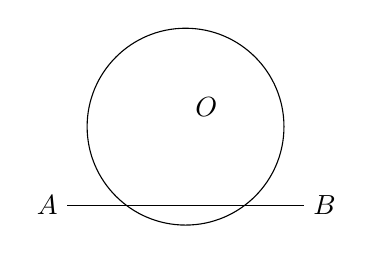
\begin{tikzpicture}[]
        % 绘制直线AB
        \coordinate [label=left:$A$] (A) at (-.5,0);
        \coordinate [label=right:$B$] (B) at (2.5,0);
        \draw (A) -- (B);
        % 标记圆心并画圆
        \coordinate [label=above right:$O$] (O) at (1,1);
        \draw (O) circle (1.25);

    \end{tikzpicture}
\end{document}